%=====================================================================
%  bar_chart_oldschool.tex   –  compile with pdflatex (twice)
%=====================================================================
\documentclass[tikz,border=5pt]{standalone}
\usepackage[T1]{fontenc}
\usepackage[utf8]{inputenc}          % needed for French accents
\usepackage{pgfplotstable}
\usepackage{pgfplots}
\pgfplotsset{compat=1.18}
\usepackage{siunitx}                 % optional, nicer y‑axis numbers
\usepackage{booktabs}                % pretty tables for the optional preview

% -------------------------------------------------
% Helper that removes the internal \pgfpl@@ wrapper
% -------------------------------------------------


\begin{document}
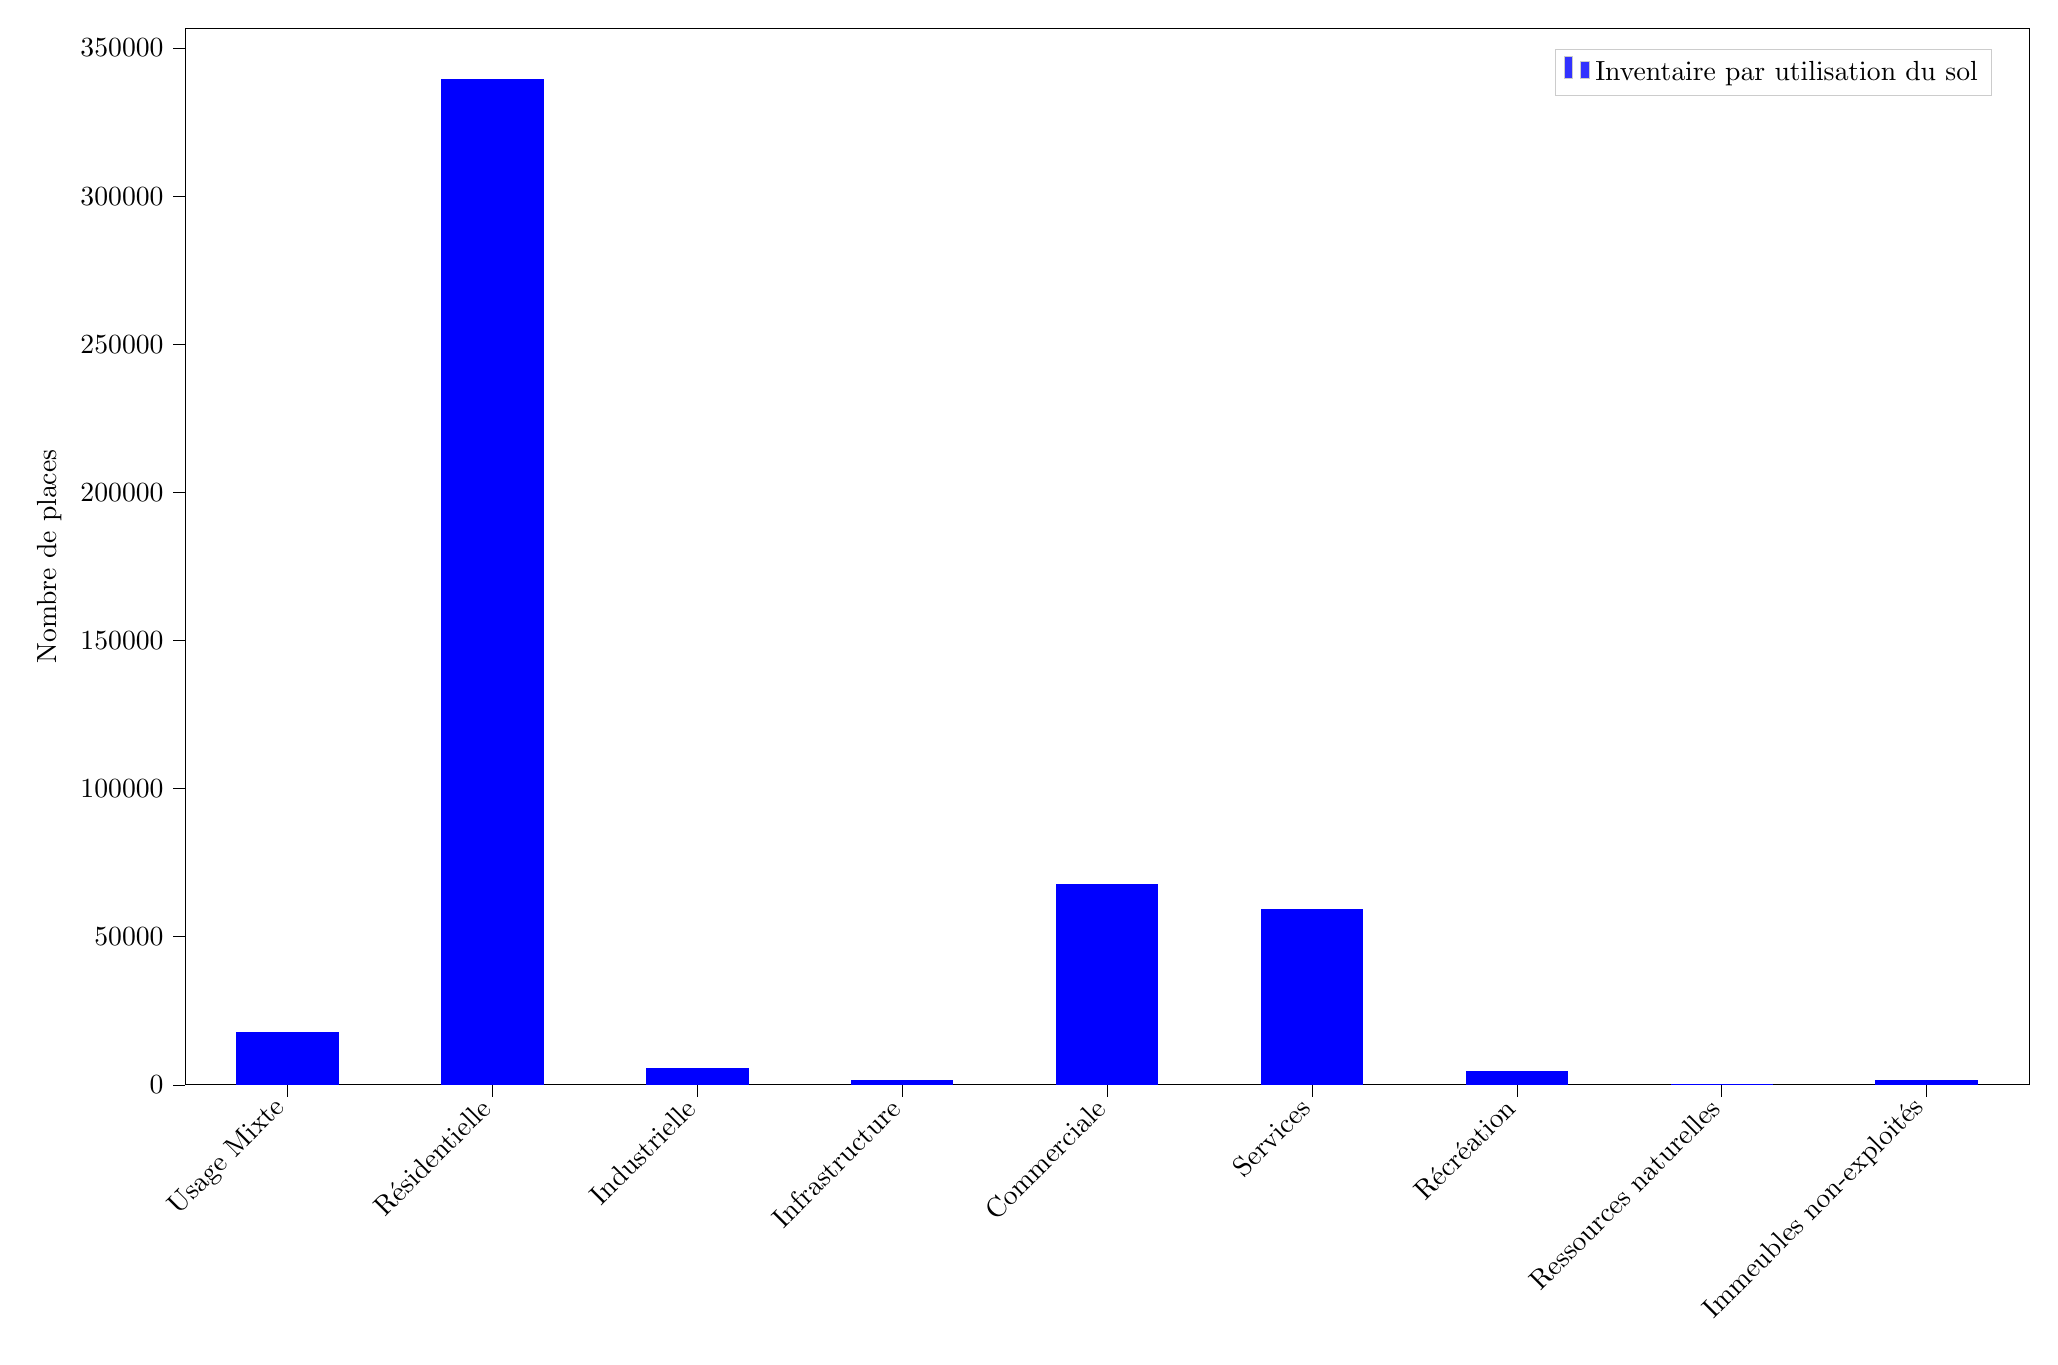
\begin{tikzpicture}

\definecolor{darkgray176}{RGB}{176,176,176}
\definecolor{lightgray204}{RGB}{204,204,204}
\definecolor{steelblue31119180}{RGB}{31,119,180}

\begin{axis}[
legend cell align={left},
legend style={fill opacity=0.8, draw opacity=1, text opacity=1, draw=lightgray204},
minor xtick={},
minor ytick={},
tick align=outside,
tick pos=left,
    height=15cm,
    width=25cm,
x grid style={darkgray176},
xmin=-0.5, xmax=8.5,
xtick style={color=black},
xtick={0,1,2,3,4,5,6,7,8},
xticklabel style={rotate=45.0,anchor=east},
xticklabels={
  Usage Mixte,
  Résidentielle,
  Industrielle,
  Infrastructure,
  Commerciale,
  Services,
  Récréation,
  Ressources naturelles,
  Immeubles non-exploités
},
y grid style={darkgray176},
ylabel={Nombre de places},
ymin=0, ymax=356673.45,
ytick style={color=black},
ytick={0,50000,100000,150000,200000,250000,300000,350000,400000},
yticklabels={
  \(\displaystyle {0}\),
  \(\displaystyle {50000}\),
  \(\displaystyle {100000}\),
  \(\displaystyle {150000}\),
  \(\displaystyle {200000}\),
  \(\displaystyle {250000}\),
  \(\displaystyle {300000}\),
  \(\displaystyle {350000}\),
  \(\displaystyle {400000}\)
},
scaled ticks= false
]
\draw[draw=none,fill=blue] (axis cs:-0.25,0) rectangle (axis cs:0.25,17709);
\addlegendimage{ybar,ybar legend,draw=none,fill=blue}
\addlegendentry{Inventaire par utilisation du sol}

\draw[draw=none,fill=blue] (axis cs:0.75,0) rectangle (axis cs:1.25,339689);
\draw[draw=none,fill=blue] (axis cs:1.75,0) rectangle (axis cs:2.25,5753);
\draw[draw=none,fill=blue] (axis cs:2.75,0) rectangle (axis cs:3.25,1731);
\draw[draw=none,fill=blue] (axis cs:3.75,0) rectangle (axis cs:4.25,67720);
\draw[draw=none,fill=blue] (axis cs:4.75,0) rectangle (axis cs:5.25,59467);
\draw[draw=none,fill=blue] (axis cs:5.75,0) rectangle (axis cs:6.25,4668);
\draw[draw=none,fill=blue] (axis cs:6.75,0) rectangle (axis cs:7.25,292);
\draw[draw=none,fill=blue] (axis cs:7.75,0) rectangle (axis cs:8.25,1785);
\end{axis}

\end{tikzpicture}




\end{document}